\documentclass[a4paper,12pt]{article}
%\documentclass[a4paper]{article}
%\documentclass{portadaUnsis}
%\usepackage[top=3cm,bottom=2cm,left=3cm,right=2cm,headsep=10pt]{geometry}
%\linespread{1.5}
\usepackage[skins,minted]{tcolorbox}
\tcbuselibrary{minted, skins}

\usepackage{wallpaper}
\usepackage{pdflscape}
\usepackage{inconsolata}
\usepackage[utf8]{inputenc}
\usepackage{listings}
%\makeatletter
%\usepackage{array}
\usepackage{setspace}
\usepackage{anysize}
\usepackage{bm}
\usepackage{textcomp}
\usepackage[T1]{fontenc}
\usepackage[spanish]{babel}
\languageshorthands{spanish}
\usepackage{multirow}
\usepackage{amsmath}
\usepackage{amsfonts}
\usepackage{color}
\usepackage{amssymb}
\usepackage{graphicx}
\usepackage{latexsym}
\usepackage{epsfig}
\usepackage{multirow}
\usepackage{fancyhdr}
\usepackage[resetfonts]{cmap}
\usepackage{lmodern}
\usepackage{hyperref}
\usepackage{url}
\usepackage{epsfig}
\usepackage{subcaption}
\usepackage{wrapfig}
\usepackage{minted}
\usepackage{xcolor}
\usepackage{color}
\usepackage{multicol}
\usepackage{multirow}
\usepackage{booktabs}
\usepackage{tabularx}
\usepackage{colortbl}
\usepackage{upquote}
\usepackage{mdframed}
\usepackage{menukeys}
\usepackage{fontawesome}
\usepackage{cite}
\usepackage{apacite}

% se usa tanto para la compilación de glosario como acrónimos
\usepackage[acronym]{glossaries}
\makeglossaries
\glossarystyle{altlistgroup}
% se incluye el archivo de definición de acrónimos
\newacronym{cpu}{CPU}{Unidad Central de Procesamiento}
% se incluye el archivo de definición de glsario
\newglossaryentry{sitioweb}{
    name=Sitio Web,
    description={Un sitio web o cibersitio es una colección de páginas web relacionadas y comunes a un dominio de internet o subdominio en la World Wide Web dentro de Internet.}
}

\definecolor{lightgray}{gray}{0.9}
\definecolor{orange}{RGB}{18,84,183}
\definecolor{titulo}{gray}{0.75}
\definecolor{gray97}{gray}{.97}
\definecolor{gray75}{gray}{.75}
\definecolor{gray45}{gray}{.45}
\definecolor{advertencia}{RGB}{255,178,102}
\definecolor{colorturqueza}{RGB}{178,223,238}
\definecolor{mintedbackground}{rgb}{0.95,0.95,0.95}
\definecolor{lbcolor}{rgb}{0.95,0.95,0.95}
\definecolor{mintedframe}{rgb}{0.0,0.0,0.0}

\lstset{
	frame=Ltb,
	tabsize=2,
	framerule=0pt,
	aboveskip=0.5cm,
	framextopmargin=0pt,
	framexbottommargin=0pt,
	framexleftmargin=0.4cm,
	framesep=0pt,
	rulesep=.0pt,
	backgroundcolor=\color{gray97},
	rulesepcolor=\color{blue},
	%
	stringstyle=\ttfamily,
	showstringspaces = false,
	basicstyle=\small\ttfamily,
	commentstyle=\color{gray45},
	keywordstyle=\bfseries,
	%
	numbers=none,
	numbersep=15pt,
	numberstyle=\tiny,
	numberfirstline = false,
	breaklines=true,
}

\setminted[bash]{
	bgcolor=mintedbackground,
	fontfamily=tt,
	linenos=true,
	numberblanklines=true,
	numbersep=11pt,
	numbersep=2pt,
	gobble=0,
	frame=leftline,
	framesep=2mm,
	funcnamehighlighting=false,
	tabsize=4,
	obeytabs=false,
	samepage=false,
	showspaces=false,
	showtabs =false,
	texcl=false,
	baselinestretch=1.2,
	fontsize=\footnotesize,
	breaklines=true,
	breaksymbolleft=\ ,
}
	 
  
% minimizar fragmentado de listados
%\lstnewenvironment{listing}[1][]{\lstset{#1}\pagebreak[0]}{\pagebreak[0]}

 
\lstdefinestyle{consola}{
	basicstyle=\footnotesize\bf\ttfamily,
	backgroundcolor=\color{gray75},
}	
\definecolor{gray}{rgb}{0.4,0.4,0.4}
\definecolor{darkblue}{rgb}{0.0,0.0,0.6}
\definecolor{cyan}{rgb}{0.0,0.6,0.6}
\lstset{language=XML}

\lstdefinelanguage{XML}{
	morestring=[b]",
	tabsize=2,
	breaklines=true,
	morestring=[s]{>}{<},
	morecomment=[s]{<?}{?>},
	stringstyle=\color{black},
	identifierstyle=\color{darkblue},
	keywordstyle=\color{cyan},
	numbers=none,
	morekeywords={xmlns,version,type}% list your attributes here
}
\lstdefinestyle{C}{language=C}
\lstdefinestyle{XML}{language=XML}
\definecolor{codebg}{rgb}{0.96,0.96,0.96}
\definecolor{colorurls}{RGB}{107,17,17}
\definecolor{colorsql}{RGB}{255,245,245}
\definecolor{colorreferences}{RGB}{48,134,3}
\definecolor{titulo}{gray}{0.65}			%------ color para fondo del titulo de tablas.
\hypersetup{
	bookmarks=true,         % show bookmarks bar?
	unicode=false,          % non-Latin characters in Acrobat’s bookmarks
	pdftoolbar=true,        % show Acrobat’s toolbar?
	pdfmenubar=true,        % show Acrobat’s menu?
	pdffitwindow=false,     % window fit to page when opened
	pdfstartview={FitH},    % fits the width of the page to the window
	pdftitle={Guía de Uso Panel HJ},    % title
	pdfauthor={Fernando Merino},     % author
	pdfsubject={Guía de Uso},   % subject of the document
	pdfcreator={pdfTeX 3.14159265-2.6-1.40.16 (TeX Live 2016/dev)},   % creator of the document
	pdfproducer={Panel HJ 2017}, % producer of the document
	pdfkeywords={mdm6} {SIG} {latex}, % list of keywords
	pdfnewwindow=true,      % links in new PDF window
	colorlinks=true,       % false: boxed links; true: colored links
	linkcolor=black,          % color of internal links (change box color with linkbordercolor)
	citecolor=colorreferences,        % color of links to bibliography
	filecolor=magenta,      % color of file links
	urlcolor=colorurls,           % color of external links
	linkbordercolor={0 0 0}
}

\lstset{literate=
	{á}{{\'a}}1 {é}{{\'e}}1 {í}{{\'i}}1 {ó}{{\'o}}1 {ú}{{\'u}}1
	{Á}{{\'A}}1 {É}{{\'E}}1 {Í}{{\'I}}1 {Ó}{{\'O}}1 {Ú}{{\'U}}1
	{à}{{\`a}}1 {è}{{\`e}}1 {ì}{{\`i}}1 {ò}{{\`o}}1 {ù}{{\`u}}1
	{À}{{\`A}}1 {È}{{\'E}}1 {Ì}{{\`I}}1 {Ò}{{\`O}}1 {Ù}{{\`U}}1
	{ä}{{\"a}}1 {ë}{{\"e}}1 {ï}{{\"i}}1 {ö}{{\"o}}1 {ü}{{\"u}}1
	{Ä}{{\"A}}1 {Ë}{{\"E}}1 {Ï}{{\"I}}1 {Ö}{{\"O}}1 {Ü}{{\"U}}1
	{â}{{\^a}}1 {ê}{{\^e}}1 {î}{{\^i}}1 {ô}{{\^o}}1 {û}{{\^u}}1
	{Â}{{\^A}}1 {Ê}{{\^E}}1 {Î}{{\^I}}1 {Ô}{{\^O}}1 {Û}{{\^U}}1
	{œ}{{\oe}}1 {Œ}{{\OE}}1 {æ}{{\ae}}1 {Æ}{{\AE}}1 {ß}{{\ss}}1
	{ç}{{\c c}}1 {Ç}{{\c C}}1 {ø}{{\o}}1 {å}{{\r a}}1 {Å}{{\r A}}1
	{€}{{\EUR}}1 {£}{{\pounds}}1 {'}{{\textquotesingle}}1 {Ñ}{{\~N}}1
	{ñ}{{\~n}}1
}

\newtcblisting{myminted}[2][]{
	listing engine=minted,
	listing only,
	#1,
	title=#2,
	minted language=bash,
	colback=mintedbackground,
	top=0mm,
	bottom=0mm
}

\newtcblisting{consolestyle}[2][]{enhanced, listing engine=minted, 
	listing only,#1, title=#2, minted language=bash, 
	coltitle=mintedbackground!35!black, 
	fonttitle=\ttfamily\footnotesize,
	sharp corners, top=0mm, bottom=0mm,
	title code={\path[draw=mintedframe, dashed, fill=mintedbackground](title.south west)--(title.south east);},
	frame code={\path[draw=mintedframe, fill=mintedbackground](frame.south west) rectangle (frame.north east);}
}


%\setlength\parindent{0pt}
\begin{document}
	\renewcommand{\tablename}{Tabla}
	\renewcommand{\figurename}{Imagen}
	\renewcommand{\listtablename}{Índice de tablas}
	\renewcommand{\listfigurename}{Índice de ilustraciones}
	\renewcommand\listoflistingscaption{Índice de códigos}
	\renewcommand\listingscaption{Código}
	
	\renewcommand*{\lstlistlistingname}{Índice de fragmentos de código}
	\renewcommand\lstlistingname{Código}
	%----------------------------------------------------------------------------------------
	%	Para la portada del documento
	%----------------------------------------------------------------------------------------
	\begingroup
	\begin{titlepage}
		\AddToShipoutPicture*{\put(0,0){
\includegraphics[scale=1]{portada/portada.pdf}}} % Image background
			\parbox[t]{1.0\linewidth}{
				\fontsize{14pt}{12pt}\selectfont
				\vspace*{0.0cm}
				 {\fontsize{20}{30}\selectfont \textcolor{white}{Plantilla Manual}}\\[2\baselineskip]
				 {\fontsize{30}{40}\selectfont \textcolor{white}{LiNuXiToS}}
				\vspace*{0.0cm}\\[2\baselineskip]
				{\fontsize{20}{30}\selectfont \textcolor{white}{Octubre 2018}\\[0.2\baselineskip]}
			}
		\begin{minipage}{\textwidth}
			\vspace{0cm}
			\noindent

			\vspace{12cm}
			\begin{flushright}
				\textcolor{white}{Creado y Desarrollado por:}\\
				\textcolor{white}{\url{https://linuxitos.com/blog/}}\\[1\baselineskip]
			\end{flushright}
			\vspace{0.2cm}
		\end{minipage}
	\end{titlepage}
	\endgroup
	%\restoregeometry

	\pagenumbering{roman}
	\pagestyle{fancy}
	\tableofcontents%
	\newpage
	\pagenumbering{arabic}
	\pagestyle{fancy}
	\lhead{Manual Developer}
	\chead{}
	\rhead{
\includegraphics[width=.2\textwidth]{img/icon-sticky-header.png}}
	
	\lfoot{
\includegraphics[width=.15\textwidth]{img/icon-sticky-header.png}}
	\cfoot{}
	\renewcommand{\footrulewidth}{0.4pt}
	\rfoot{Pág. \thepage}
	\section{Manuales de usuario}

En los manuales de usuarios, se utiliza glosarios \verb|\gls{sitioweb}| = \gls{sitioweb}  acrónimos como \verb|\acrfull{cpu}| = \acrfull{cpu} o citas biblíográficas, en casos raros \verb|\cite{boria}| = \cite{boria}, pero también se utilizan.

\begin{figure}[!htb]
	\centering
	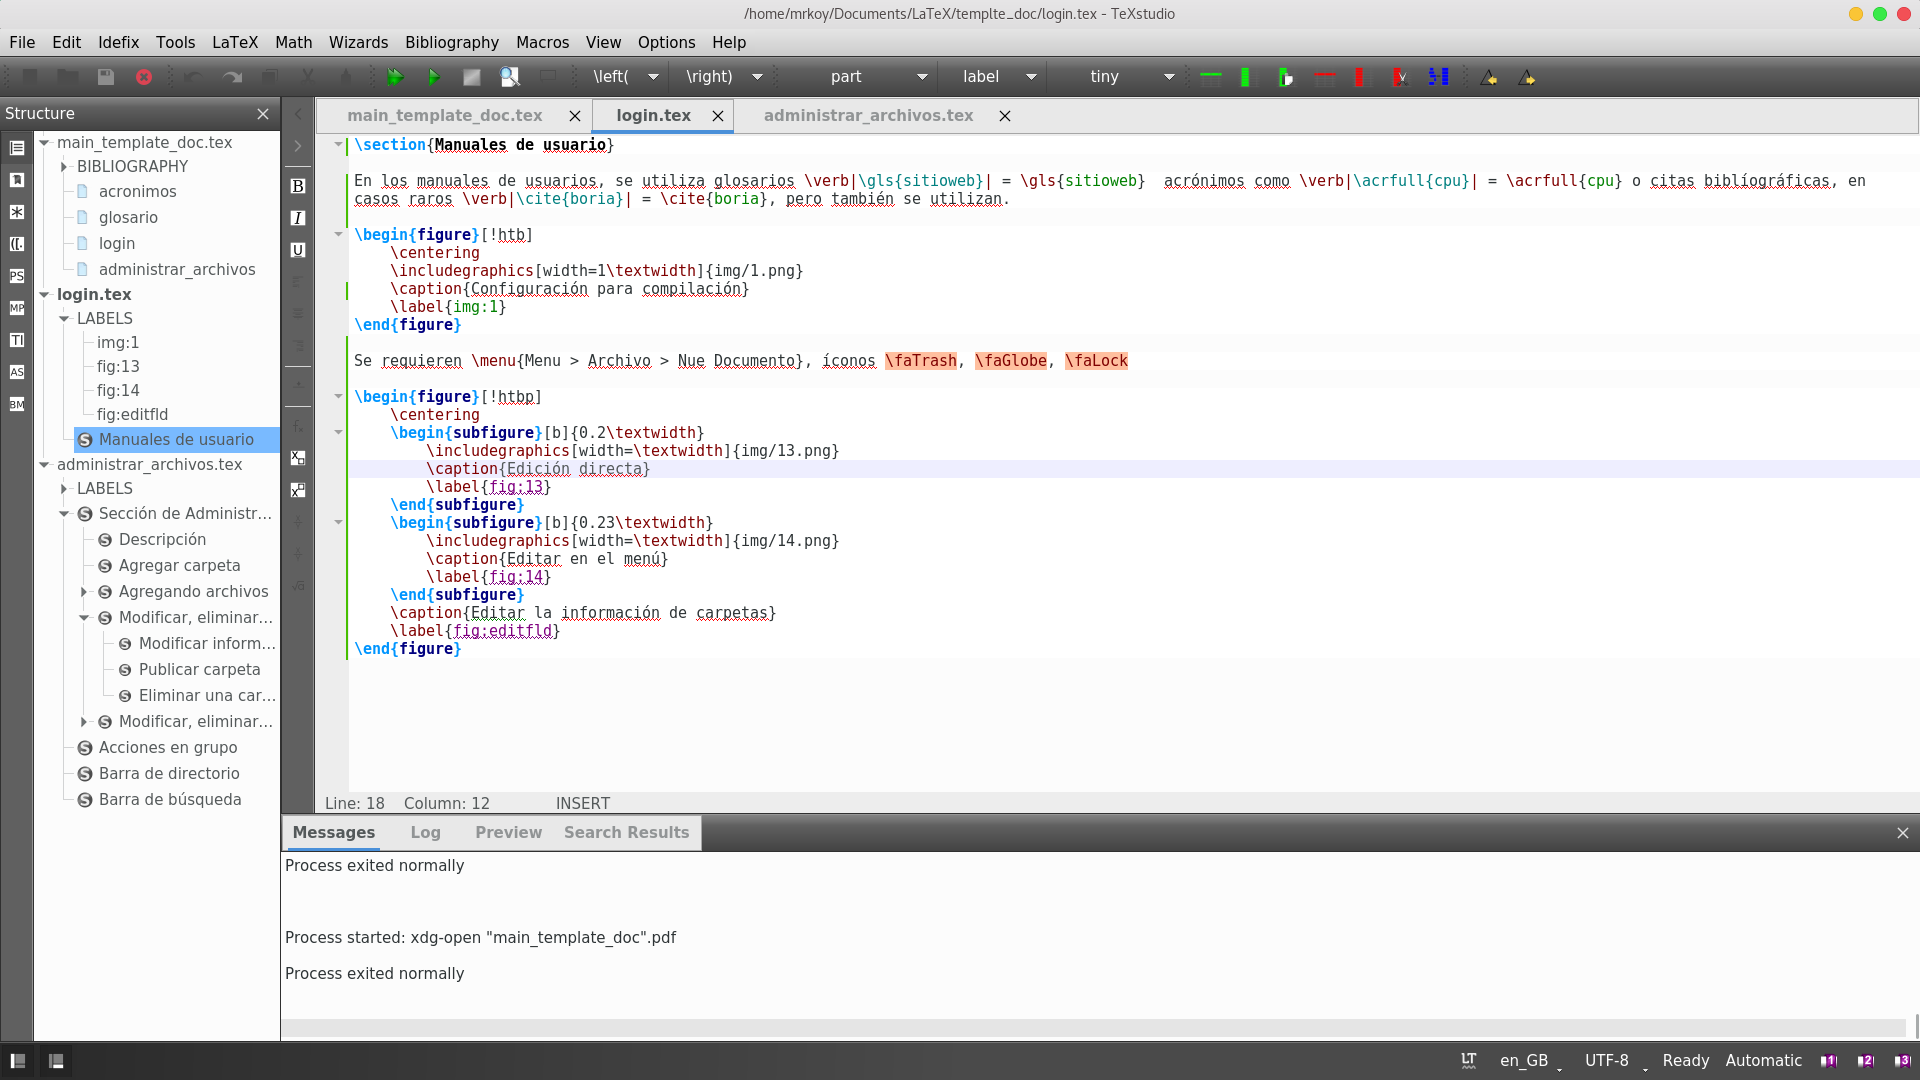
\includegraphics[width=1\textwidth]{img/3.png}
	\caption{TexStudio}
	\label{img:1}
\end{figure}

Se requieren \menu{Menu > Archivo > Nuevo Documento}, íconos \faTrash, \faGlobe, \faLock

\begin{figure}[!htbp]
	\centering
	\begin{subfigure}[b]{0.41\textwidth}
		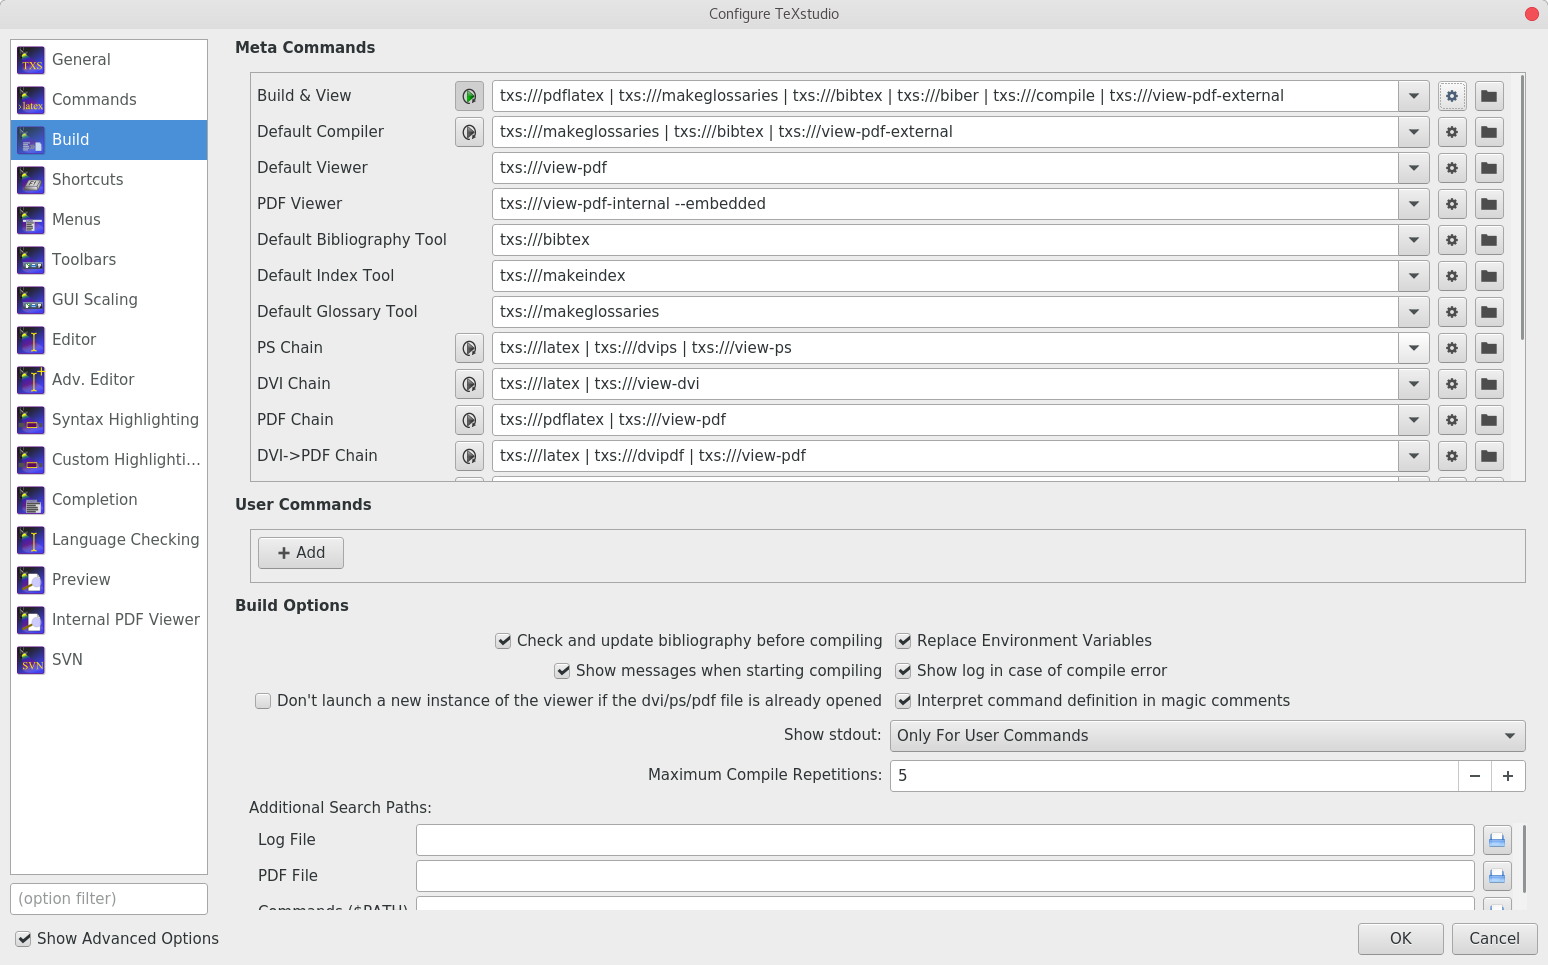
\includegraphics[width=\textwidth]{img/1.png}
		\caption{Configuración}
		\label{fig:2}
	\end{subfigure}
	\begin{subfigure}[b]{0.52\textwidth}
		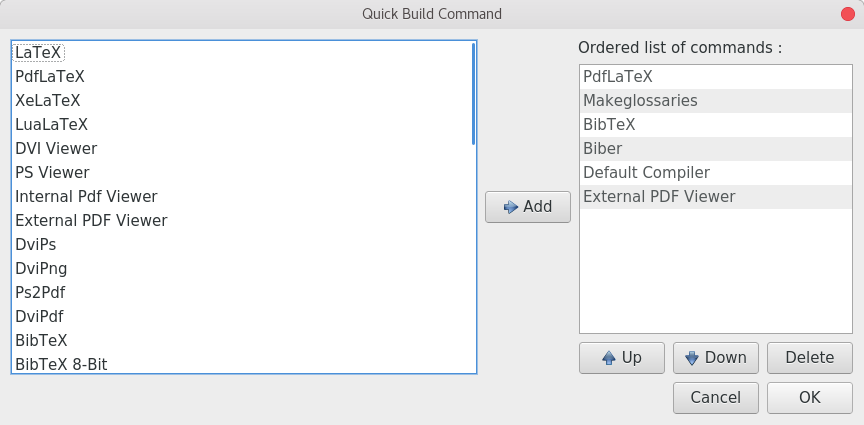
\includegraphics[width=\textwidth]{img/2.png}
		\caption{Orden de compilación}
		\label{fig:3}
	\end{subfigure}
	\caption{Configuración para compilación}
	\label{fig:compile}
\end{figure}

\section{Códigos}

Sin duda alguna habrá fragmentos de código:

\begin{mdframed}[linecolor=black, topline=false, bottomline=false, leftline=false, rightline=false, userdefinedwidth=\textwidth]
\captionof{lstlisting}{Fragmentos de código}
\label{cod:gauss}
\vspace{-0.3cm} %separción entre el caption y el código
\begin{minted}[mathescape, breaklines, frame=single, tabsize=4, gobble=0, linenos, numbersep=5pt,]{c}
////////////////////////////////////////////////
// Función de membresía Guassiana 
//$f(x)=e^{-\alpha \frac{x - c}{\delta}^2}$
////////////////////////////////////////////////

double gaussiana(double centro, double ancho, double x){
	double ux=0;
	ux=pow(2.718281828, ( -.5* pow(((x-centro) / ancho), 2)));
	return ux;
}
\end{minted}
\end{mdframed}

\section{Imágenes}
Una de las principales características de los manuales, es que llevan muchas imágenes, muchas [...]

\begin{figure}[!htb]
	\centering
	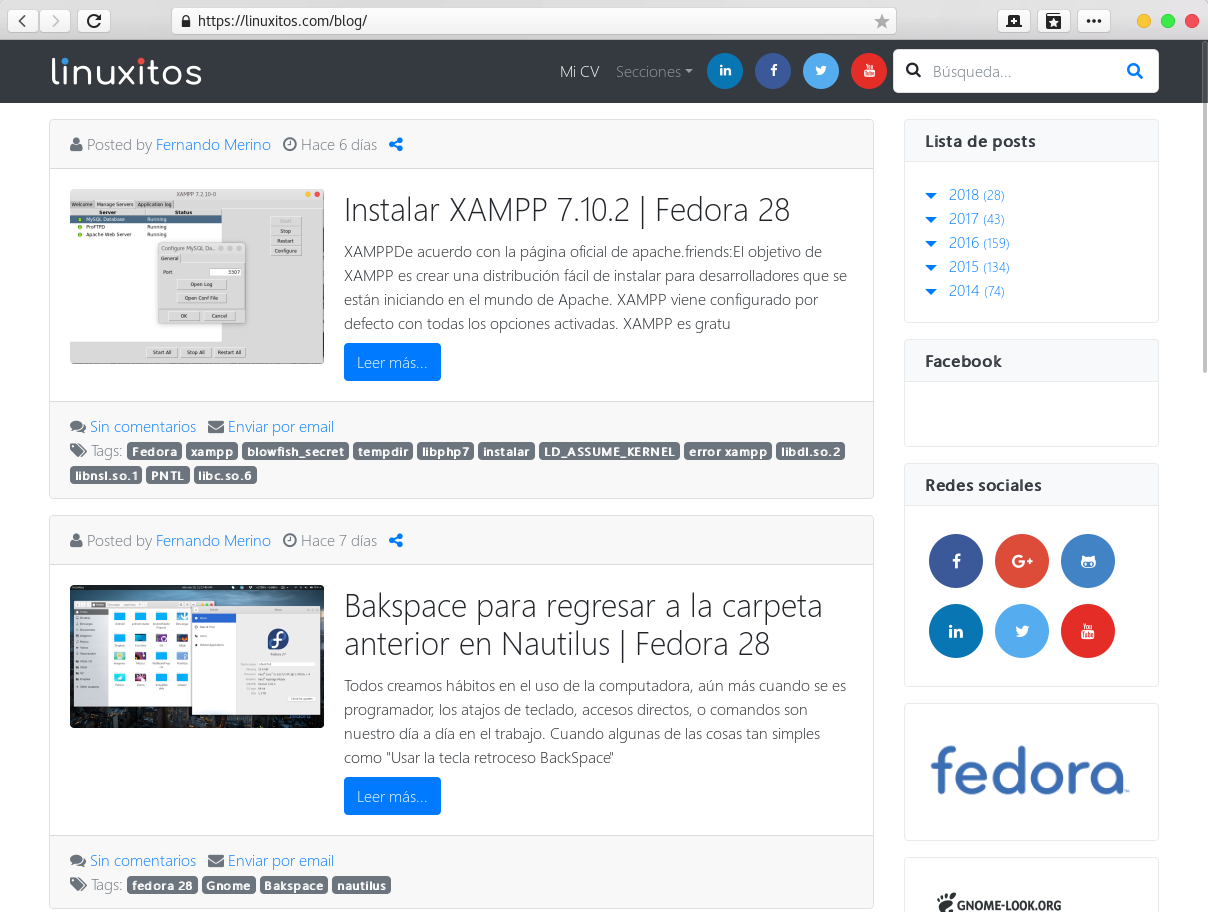
\includegraphics[width=1\textwidth]{img/4.png}
	\caption{\url{https://linuxitos.com/blog/}}
	\label{img:4}
\end{figure}

\section{Terminal}
Si es un manual sobre linux, entonces, habrá fragmentos de comandos:

\begin{myminted}{Terminal}
	sudo dnf -y install evince gedit zip file-roller xz lzma
\end{myminted}





		
	\rfoot{Pág. \thepage}
	
	\pagestyle{fancy}
	\lhead{Apéndices}
	\chead{}
	\rhead{
\includegraphics[width=.123\textwidth]{img/icon-sticky-header.png}}
	
	\lfoot{LiNuXiToS}
	\cfoot{}
	\renewcommand{\footrulewidth}{0.4pt}
	\rfoot{Pág. \thepage}
	\rfoot{Pág. \thepage}
	
	\newpage
	\printglossary[title=Glosario,toctitle=Glosario]
	%linea que anexa la palbra Glosario al índice
	\addcontentsline{toc}{section}{Glosario}
	
	\newpage
	\printglossary[type=\acronymtype]
	%linea que anexa la palbra Acrónimo al índice
	\addcontentsline{toc}{section}{Acrónimos}

	
	\newpage
	\bibliography{bibliografia}
	\bibliographystyle{apacite}
\end{document}